\documentclass[../rapport_MVEX01-11-05]{subfiles}
\begin{document}

\subsection{Egenskaper}\label{sec:resultat_features}

\notes{Någon inledande bullshit-text?}

\subsubsection{Observationer i egenskapsrumet}

\notes{förklara vilka som ser ut
att fungera bäst för att urskilja gester.}
För att \knn-metoden enklare ska kunna klassificera gester är det viktigt att
egenskapsrummet är utformat så att bilder från varje gest är både tydligt
separerade och tydligt grupperade. Det viktigaste är grupperingen; att gester
är separerade är något som endast förenklar processen.

Trots att gesterna ligger mycket tätt i egenskapsrummet så är de redan i det
tvådimensionella underrummet till egenskapsrummet som visas i figur~\ref{fig:feats1011}
mycket tydligt grupperade, vilket gör att \knn-metoden ger exakta resultat.

\begin{figure}[htb]
  \centering
  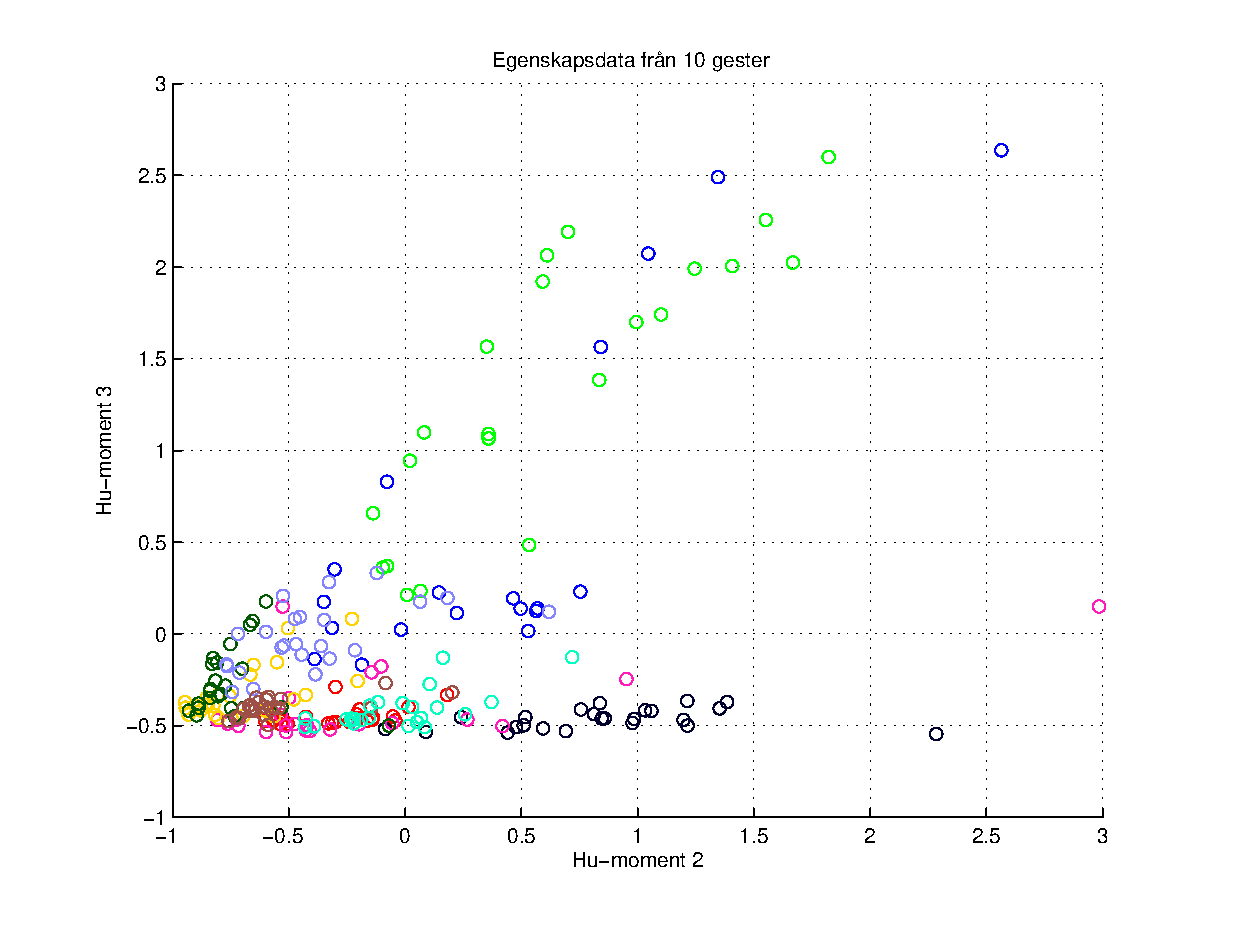
\includegraphics[width=\textwidth]{bilder/feats-10+11}
  \caption{Andra och tredje Hu-momenten för prototypdatan}
  \label{fig:feats1011}
\end{figure}

Fler egenskaper än de två i figur~\ref{fig:feats1011} ger inte helt oväntat
(men inte heller trivialt) ett bättre resultat. Figur~\ref{fig:knnplot} visar
hur det relativa felet minskar både då $k$ ökar i \knn-metoden och då antalet
egenskaper som inkluderas i rummet ökar. Något mer oväntat är dock att det
finns ett tydligt minimum som inte inkluderar alla egenskaper.

\end{document}